\chapter{Options}
\section{Introduction}

\begin{itemize}
    \item Discuss why firms have a risk management policy
    \item Explain the mechanics of the options market and pricing
    \item Produce a payoff at maturity chart
    \item Describe the put-call parity relationship.
\end{itemize}

\section{Options}

\begin{itemize}
    \item Options are prevalent in financial markets and trading strategies.
    \item Three key terms: 'in the money', 'at the money', and 'out of the money' categorize options based on the relationship between the underlying asset's price and the strike price.
\end{itemize}

\subsection*{European Call and Put Options}

\begin{itemize}
    \item European call option: Gives the holder the right to buy the underlying asset at a pre-specified price (strike price) on a predetermined future date (expiry date).
    \item European put option: Grants the owner the right to sell the underlying asset at the strike price on the expiry date.
    \item European options can only be exercised at the expiry date, unlike American options which offer flexibility for early exercise.
    \item The price paid for an option is called the option's premium.
\end{itemize}

\subsection*{Option Categories}

\begin{itemize}
    \item \textbf{In the Money (ITM)}: When the option's intrinsic value is positive because the asset's price is significantly higher (for calls) or lower (for puts) than the strike price. 
    \item \textbf{Out of the Money (OTM)}: When the option's intrinsic value is zero because the asset's price is well below (for calls) or above (for puts) the strike price.
    \item \textbf{At the Money (ATM)}: When the asset's price is close to the strike price. In this region, the speculative value of the option is the primary driver of its price.
\end{itemize}

\subsection*{Value Components of Options}

\begin{itemize}
    \item \textbf{Intrinsic Value}: Only present in ITM options. Represents the difference between the option's exercise price and the spot (current) price of the underlying asset. \textbf{In other words, it is the value of the option if it were to be exercised immediately.}
    \item \textbf{Speculative Value}: The difference between the option's premium and its intrinsic value. ATM and OTM values have zero intrinsic value, so it's equal to the option premium in the case of ATM or OTM. It is influenced by volatility, it is the primary component of at-the-money options (since options become more volatile as they approach the strike price).
\end{itemize}


\begin{examplebox}{Options Questions}
    \textbf{Question 1:} Suppose you have purchased a call option with a strike price of \$50.00 and a premium of \$3.00, and that the current stock price is \$54.00 at expiration. Calculate the payoff of the long call option.

\textbf{Answer:} The payoff of the long call option is $\text{Max}(S - K, 0) - P = \text{Max}(54 - 50, 0) - 3 = 1$\\

\textbf{Question 2:} Suppose you have written (shorted) a call option with a strike price of \$60.00, received a premium of \$5.00, and that the stock price at expiration is \$58.00. Calculate the payoff of the short call option.

\textbf{Answer:} The payoff of the short call option is $-[\text{Max}(S - K, 0) - P] = -[\text{Max}(58 - 60, 0) - 5] = 5$\\

\textbf{Question 3:} Assume you have purchased a put option with a strike price of \$85.00 and a premium of \$6.00, and that the stock price at expiration is \$90.00. Calculate the payoff of the long put option.

\textbf{Answer:} The payoff of the long put option is $\text{Max}(K - S, 0) - P = \text{Max}(85 - 90, 0) - 6 = -6$\\

\textbf{Question 4:} You have sold (shorted) a put option with a strike price of \$75.00, received a premium of \$4.00, and the stock price at expiration is \$70.00. Calculate the payoff of the short put option.

\textbf{Answer:} The payoff of the short put option is $-[\text{Max}(K - S, 0) - P] = -[\text{Max}(75 - 70, 0) - 4] = -1$\\
\end{examplebox}

\section{Options Payoff Structures}

Options trading involves the agreement between two parties to facilitate the potential transaction on an underlying security at a predetermined price, known as the strike price (\(K\)), before a specified date. The buyer of the option acquires the right, but not the obligation, to execute the transaction.

\subsection*{Long Call}

A long call option gives the holder the right to buy the underlying asset at the strike price (\(K\)). The payoff for a long call option is given by:
\[ \text{Payoff} = \max(0, S_T - K)-\text{premium} \]
where \( S_T \) is the price of the underlying asset at maturity.\\

\textbf{Example:} Consider a long call option with a premium of 10, with a strike price of \( K = 100 \). If at maturity, the asset price is \( S_T = 120 \), the payoff is \( \max(0, 120 - 100) -10 = 10 \).

\begin{figure}[H]
    \centering
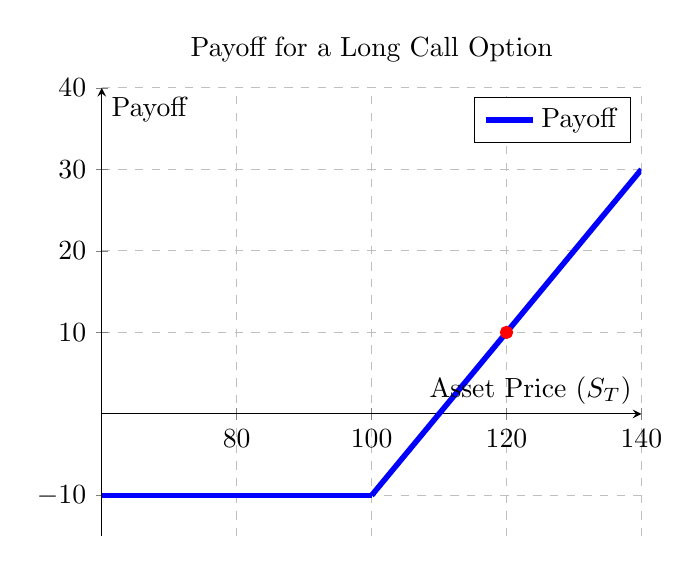
\begin{tikzpicture}
\begin{axis}[
    title={Payoff for a Long Call Option},
    xlabel={Asset Price (\( S_T \))},
    ylabel={Payoff},
    xmin=60, xmax=140,
    ymin=-15, ymax=40,
    axis lines=middle,
    grid=major,
    grid style=dashed,
]
\addplot[blue, thick,line width=2pt, domain=100:140]{max(0, x-100)-10};
\addplot[blue, thick,line width=2pt, domain=60:100]{-10};

%  add a dot to (120, 10)
\addplot[red, mark=*, thick] coordinates {(120, 10)};

\legend{Payoff}
\end{axis}
\end{tikzpicture}
\end{figure}

\subsection*{Short Call}

A short call option involves selling the call option, thus obligating the seller to sell the underlying asset at the strike price if the option is exercised. The payoff for a short call option is:
\[ \text{Payoff} = \min(0, K - S_T) + \text{premium} \]

\textbf{Example:} If a short call option with premium 10 and a strike price of \( K = 100 \) is exercised and the asset price is \( S_T = 120 \), the payoff is \( \min(0, 100 - 120) + 10 = -10 \).

\begin{figure}[H]
    \centering
    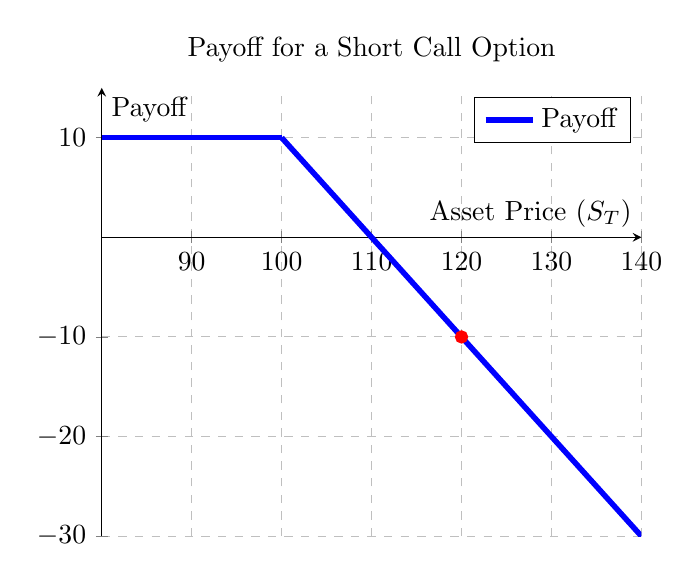
\begin{tikzpicture}
        \begin{axis}[
            title={Payoff for a Short Call Option},
            xlabel={Asset Price (\( S_T \))},
            ylabel={Payoff},
            xmin=80, xmax=140,
            ymin=-30, ymax=15,
            axis lines=middle,
            grid=major,
            grid style=dashed,
        ]
        \addplot[blue, thick,line width=2pt, domain=100:140]{min(0, 100-x)+10};
        \addplot[blue, thick,line width=2pt, domain=80:100]{10};
        \addplot[red, mark=*, thick] coordinates {(120, -10)};
        \legend{Payoff}
        \end{axis}
        \end{tikzpicture}
\end{figure}

\subsection*{Long Put}

A long put option gives the holder the right to sell the underlying asset at the strike price. The payoff for a long put option is:
\[ \text{Payoff} = \max(0, K - S_T) - \text{premium}\]

\textbf{Example:} For a long put option with a premium of 10 and a strike price of \( K = 100 \) and an asset price at maturity of \( S_T = 80 \), the payoff is \( \max(0, 100 - 80) -10 = 10 \).

\begin{figure}[H]
    \centering
    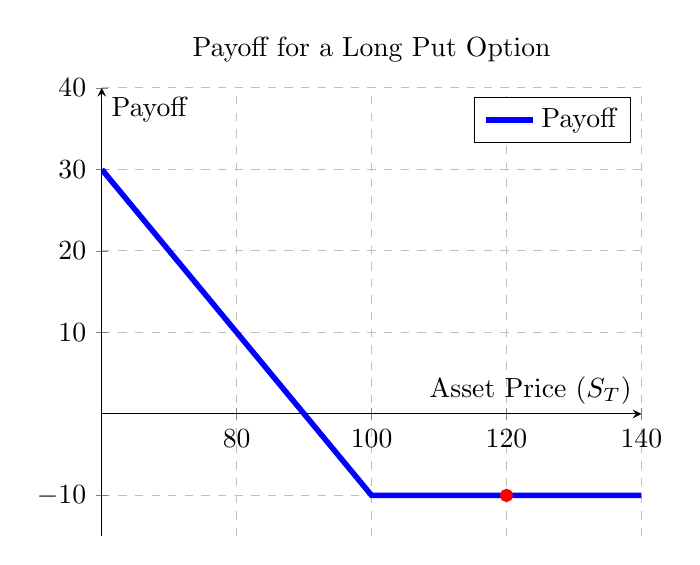
\begin{tikzpicture}
        \begin{axis}[
            title={Payoff for a Long Put Option},
            xlabel={Asset Price (\( S_T \))},
            ylabel={Payoff},
            xmin=60, xmax=140,
            ymin=-15, ymax=40,
            axis lines=middle,
            grid=major,
            grid style=dashed,
        ]
        \addplot[blue, thick,line width=2pt, domain=60:140]{max(0, 100-x)-10};
        \addplot[red, mark=*, thick] coordinates {(120, -10)};
        \legend{Payoff}
        \end{axis}
        \end{tikzpicture}
\end{figure}

\subsection*{Short Put}

A short put option involves selling the put option, obligating the seller to buy the underlying asset at the strike price if the option is exercised. The payoff for a short put option is:
\[ \text{Payoff} = \min(0, S_T - K) + \text{premium} \]

\textbf{Example:} If a short put option with a strike price of \( K = 100 \) is exercised and the asset price at maturity is \( S_T = 80 \), the payoff is \( \min(0, 80 - 100)  + 10= 10\).

\begin{figure}[H]
    \centering
    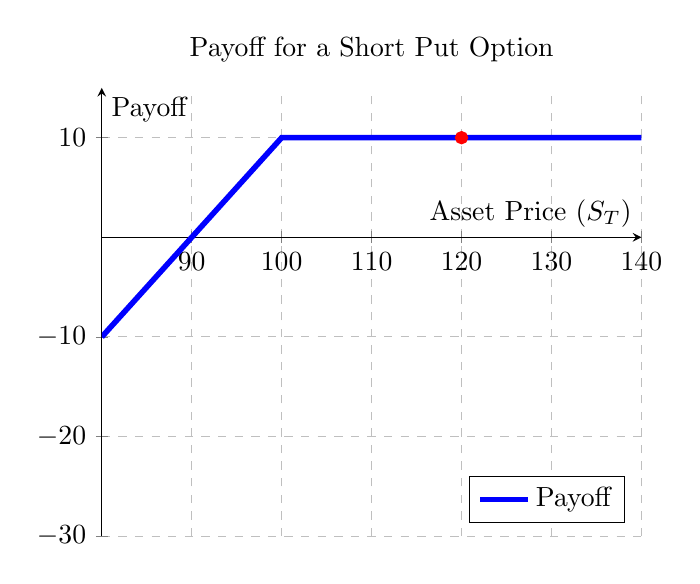
\begin{tikzpicture}
        \begin{axis}[
            title={Payoff for a Short Put Option},
            xlabel={Asset Price (\( S_T \))},
            ylabel={Payoff},
            xmin=80, xmax=140,
            ymin=-30, ymax=15,
            axis lines=middle,
            grid=major,
            grid style=dashed,
            legend pos = south east,
        ]
        \addplot[blue, thick, line width = 2pt, domain=80:140]{min(0, x-100) + 10};
        \addplot[red, mark=*, thick] coordinates {(120, 10)};


        \legend{Payoff}
        \end{axis}
        \end{tikzpicture}
\end{figure}

Out of all four cases, it was only the short put that had a positive payoff. 

\section{Binomial Option Pricing Model}

The Binomial Model assumes that in each period (time step), the return of the underlying asset can take one of two possible values.

\begin{figure}[H]
    \centering
    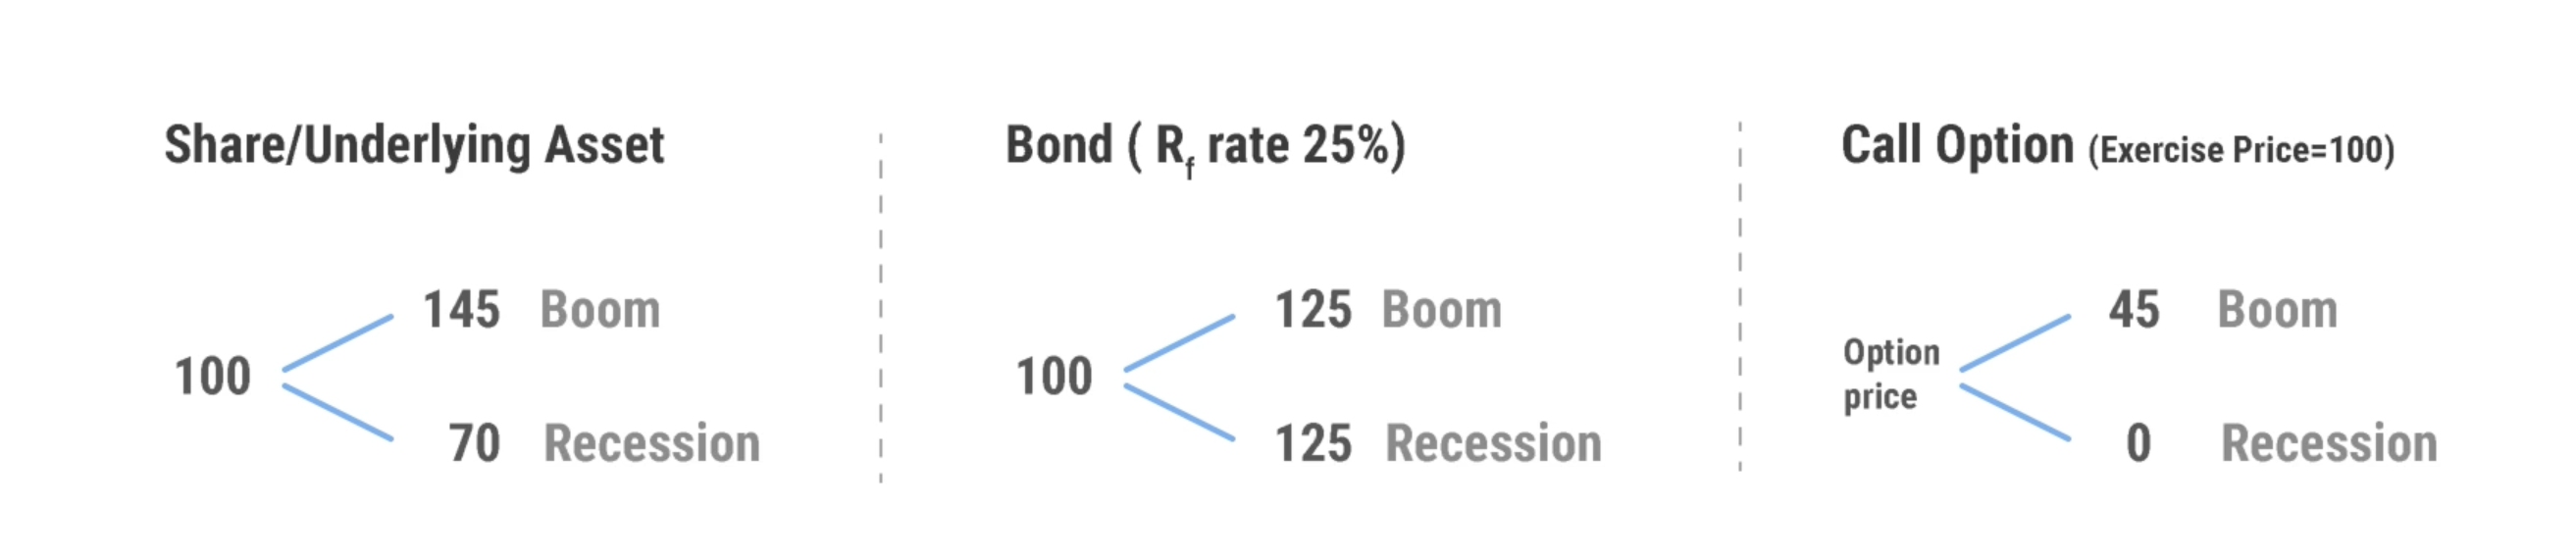
\includegraphics[width=0.9\textwidth]{img/9.4.1.png}
    \caption{Binomial valuation of options}
    \label{fig:binomial}
\end{figure}

\subsection*{Replication}
A replication strategy finds an investment in a combination of asset and risk-free bond (for calculation purposes, assume the bond is always risk-free) that replicates the call option's payoff at maturity.  To do this we need to determine the call option's delta, the number of shares needed in the replicating portfolio to replicate the option's payoff.

We have the following equations:

\begin{align}
    \text{Upwards movement in share price: } uS\Delta + (1+r_f)B &= C^{up}\\
    \text{Downwards movement in share price: } dS\Delta + (1+r_f)B &= C^{down}
\end{align}

\begin{itemize}
    \item Where \( u \) and \( d \) are the upward and downward multiplied movements in the share price, so $uS$ and $dS$ are the final share prices in the up and down states.
    \item \( S \) is the current share price,
    \item \( \Delta \) is the number of shares in the replicating portfolio,
    \item \( B \) is the amount invested in the risk-free bond,
    \item \( r_f \) is the risk-free rate, and
    \item \( C^{up} \) and \( C^{down} \) are the call option prices in the up and down states, respectively.
\end{itemize}

We can solve the equations to find the replicating portfolio's delta and the amount invested in the risk-free bond. From this point onwards, $r$ refers to the risk-free rate.

\begin{align}
    \Delta&=\frac{C^{up}-C_{\mathrm{down}}}{(u-d)S}\\
    B     &=\frac{uC_{\mathrm{down}}-dC^{up}}{(u-d)(1+r_f)}
\end{align}

The call option price $C$ is the delta times the share price plus the amount invested in the risk-free bond.

\begin{equation}
    C = S\Delta + B
\end{equation}

Solving the example in Figure \ref{fig:binomial}, we have:

\begin{align*}
    &\Delta=0.6 \\
    &B=-33.6 \\
    &C=0.6 \times 100 - 33.6 = 26.4
    \end{align*}

\subsection*{Risk-Neutral Model}

This stems from the replicating portfolio method, but also determines the risk-neutral probabilities of the two outcomes, for example, a boom or recession in the example of Figure \ref{fig:binomial}.\\

When these probabilities have been determined, we discount the expected payoff of the option at the risk-free rate.\\

The price of the call option can be expressed as the present value of the expected payoff,

\begin{equation}
    C = \frac{pC^{up}+(1-p)C^{down}}{r}
\end{equation}

Where $r$ is the risk-free rate and $p$ is the risk-neutral probability of the upward movement. $p$ is defined by:


\begin{equation}
    p = \frac{1+r-d}{u-d}
\end{equation}

Where:
\begin{itemize}
    \item \( r \) is the risk-free rate,
    \item \( u \) is the upward movement in the share price, and
    \item \( d \) is the downward movement in the share price.
\end{itemize}

In the example of Figure \ref{fig:binomial}, we have:
\begin{align}
    p=\frac{1.25-0.7}{1.45-0.7}=0.733\\
    1-p = 0.267
\end{align}

We can extend this model to a two-period example, reusing the values for $d$ and $u$.
\begin{figure}[H]
    \centering
    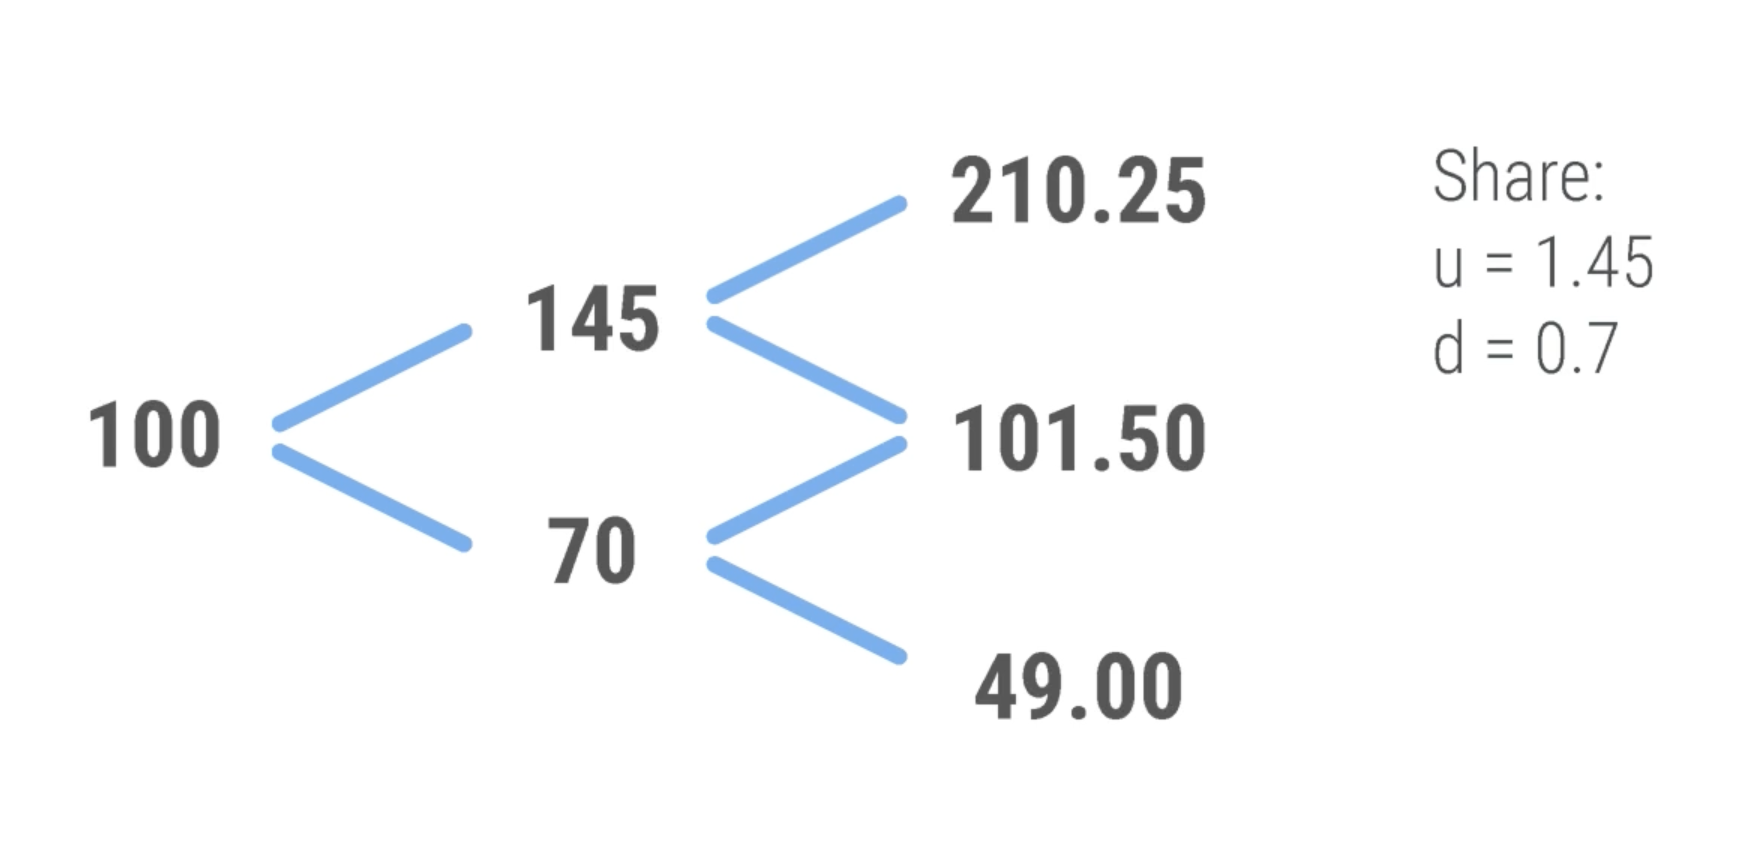
\includegraphics[width=0.5\textwidth]{img/9.4.2.png}
    \caption{Two-period binomial model (stock tree)}
    \label{fig:two-period}  
\end{figure}

In the case of only being provided only the final outcomes, it is non-trivial to determine the prices in different points in time, since the values of $u$ and $d$ are the same for every time step.

\begin{figure}[H]
    \centering
    \begin{subfigure}{0.48\textwidth}
        \centering
        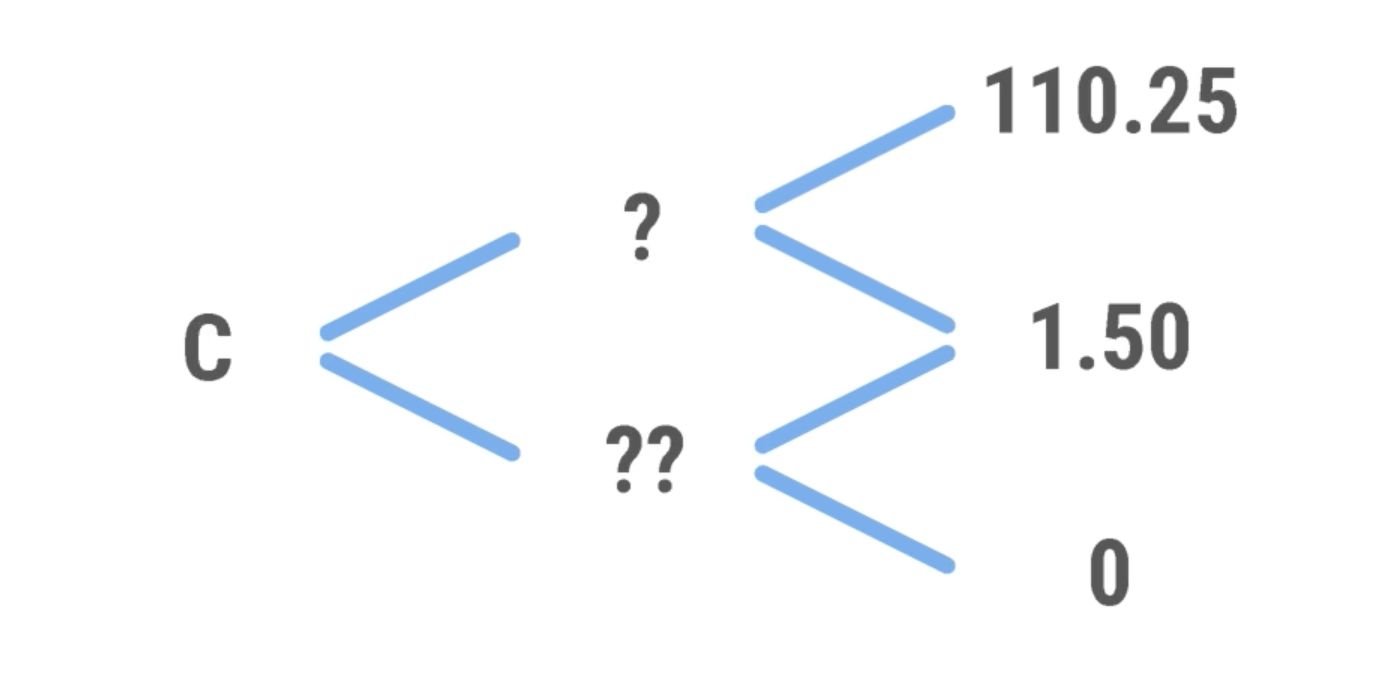
\includegraphics[width=0.5\textwidth]{img/9.4.3.png}
    \end{subfigure}
    \begin{subfigure}{0.48\textwidth}
        \centering
        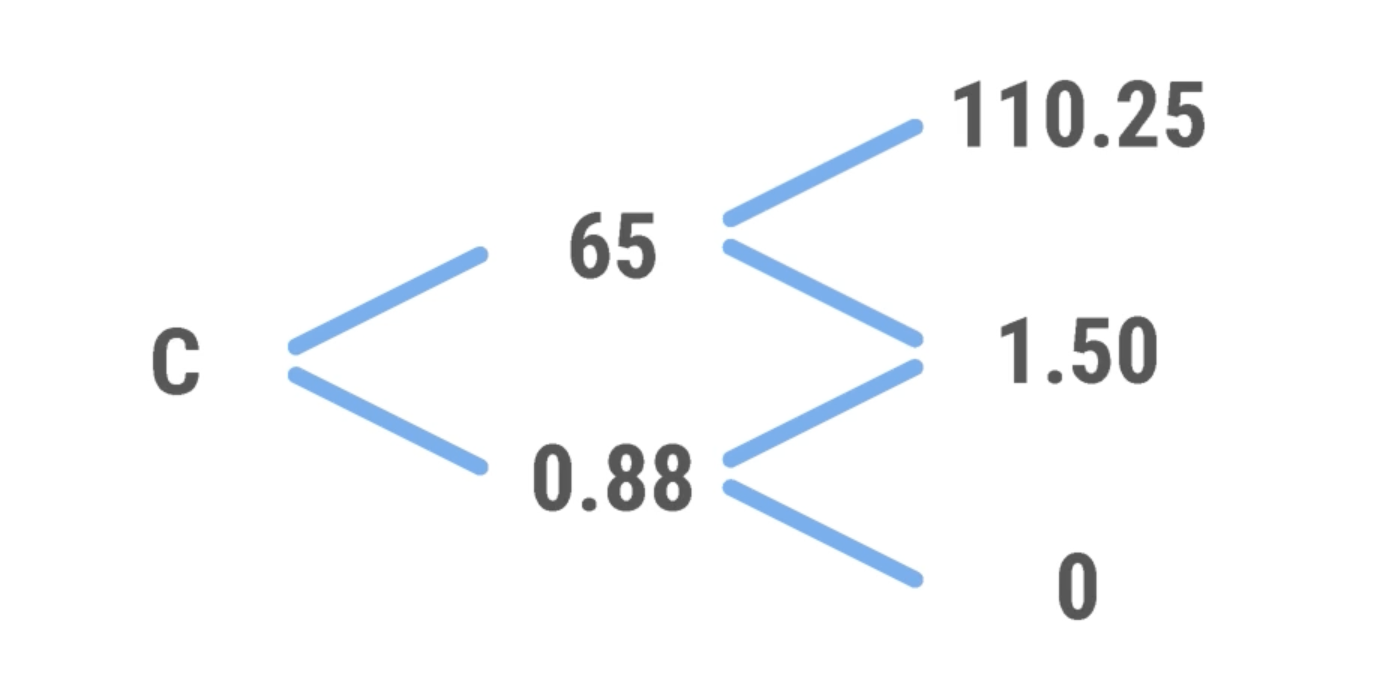
\includegraphics[width=0.5\textwidth]{img/9.4.4.png}
    \end{subfigure}
    \caption{Determining prices in a two-period binomial model (stock tree)}
\end{figure}

\subsection*{Put-Call Parity}
Put-call parity is a relationship between the price of a European call option and a European put option with the same strike price and expiry date. It is given by:

\begin{equation}
    C - P = S - Ke^{-rT}
\end{equation}
    
    Where:
    \begin{itemize}
        \item \( C \) is the price of the call option,
        \item \( P \) is the price of the put option,
        \item \( S \) is the current price of the underlying asset,
        \item \( K \) is the strike price of the options,
        \item \( r \) is the risk-free rate, and
        \item \( T \) is the time to maturity.
    \end{itemize}   



\begin{examplebox}{Options Questions}

\begin{figure}[H]
    \centering
    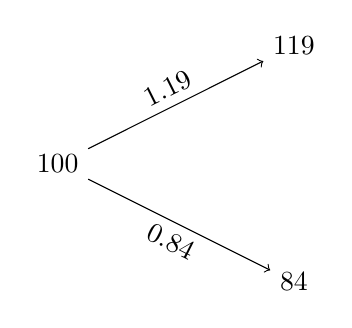
\begin{tikzpicture}[sloped]
        \node (a) at (0,0) {$100$};
        \node (b) at (3,-1.5) {$84$};
        \node (c) at (3,1.5) {$119$};

        
        \draw [->] (a) to node [below] {$0.84$} (b);
        \draw [->] (a) to node [above] {$1.19$} (c);
      \end{tikzpicture}
      \caption{Stock Tree}
\end{figure}

      
    \textbf{Question:} Over the next year, the price of stock W could increase by 19\% or go down by 16\%. Currently, the value of a stock is 100. The annual riskless interest rate is 4\%. What is the risk-neutral probability of the scenario (state) `up'?\\

\textbf{Answer:}
Using the formula for the risk-neutral probability:
\[
p = \frac{1 + r - d}{u - d}
\]
where \( r = 0.04 \) (risk-free rate), \( u = 1.19 \) (up movement), and \( d = 0.84 \) (down movement), we calculate:
\[
p = \frac{1.04 - 0.84}{1.19 - 0.84} = \frac{0.20}{0.35} \approx 0.57
\]

\textbf{Question:} What is the value of a European call option on a share of company W, with an exercise price of 90 and time to maturity of 1 year?\\

\textbf{Answer:}
Assuming that the strike price \( K = 90 \), and using the previously calculated risk-neutral probability \( p = 0.57 \), the values in the up and down state at maturity would be:
\[
C^{up} = \max(0, 1.19 \times 100 - 90) = 29
\]
\[
C^{down} = \max(0, 0.84 \times 100 - 90) = 0
\]

The option will not be exercised at the down state as 84 is less than 90. So the option value is 0. Using the equation:
\begin{equation}
    C = \frac{pC^{up}+(1-p)C^{down}}{r}
\end{equation}

We work out the option's current value to be:
\[
C = \frac{0.57 \times 29 + 0.43 \times 0}{1.04} \approx 15.894
\]

\begin{figure}[H]
    \centering
    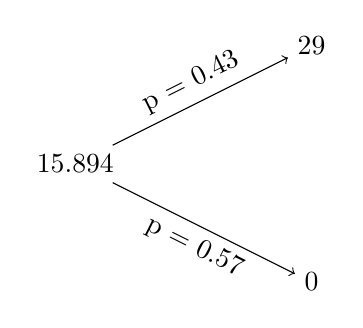
\begin{tikzpicture}[sloped]
        \node (a) at (0,0) {$15.894$ };
        \node (b) at (3,-1.5) {$0$};
        \node (c) at (3,1.5) {$29$};

        
        \draw [->] (a) to node [below] {p = 0.57} (b);
        \draw [->] (a) to node [above] {p = 0.43} (c);
      \end{tikzpicture}
      \caption{Call Tree}
\end{figure}

The option value \( C \) is then:
\[
C = \frac{0.57 \times 29 + 0.43 \times 0}{1.04} \approx 15.894
\]

\textbf{Question:} Based on put-call parity, compute the value of a put option on stock W, with time to maturity of 1 year and a strike price of 90.\\

\textbf{Answer:}
Using put-call parity:
\[
P = C + Ke^{-rT} - S
\]
Substituting the values:
\[
P = 15.894 + 90e^{-0.04 \times 1} - 100
\]
\[
P \approx 2.37
\]

\textbf{Question:} Determine the value of a put option on stock W with time to maturity of 2 years and an exercise price of 90.\\

\textbf{Answer:}
This question requires extending the binomial model to two periods. To fill in the 1st period on the call tree, use the equation:

\begin{equation}
    C = \frac{pC^{up}+(1-p)C^{down}}{r}
\end{equation}

\begin{figure}[H]
    \centering
    \begin{subfigure}[b]{0.48\textwidth}
        \centering
        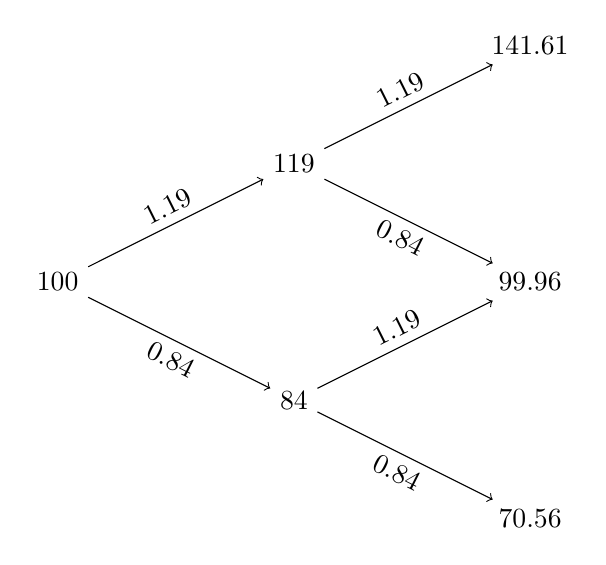
\begin{tikzpicture}[sloped]
            \node (a) at (0,0) {$100$};
            \node (b) at (3,-1.5) {$84$};
            \node (c) at (3,1.5) {$119$};
            \node (d) at (6,-3) {$70.56$};
            \node (e) at (6,0) {$99.96$};
            \node (f) at (6,3) {$141.61$};
            
            \draw [->] (a) to node [below] {$0.84$} (b);
            \draw [->] (a) to node [above] {$1.19$} (c);
            \draw [->] (c) to node [below] {$0.84$} (e);
            \draw [->] (c) to node [above] {$1.19$} (f);
            \draw [->] (b) to node [below] {$0.84$} (d);
            \draw [->] (b) to node [above] {$1.19$} (e);
        \end{tikzpicture}
        \caption{Stock Tree}
    \end{subfigure}
    \begin{subfigure}[b]{0.48\textwidth}
        \centering
        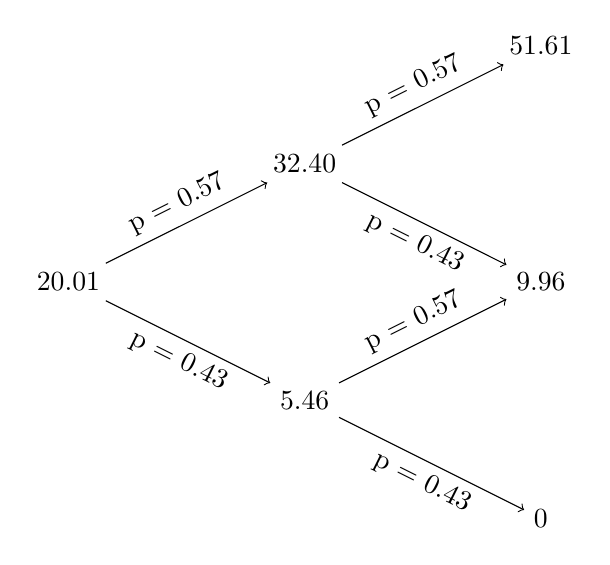
\begin{tikzpicture}[sloped]
            \node (a) at (0,0) {$20.01$};
            \node (b) at (3,-1.5) {$5.46$};
            \node (c) at (3,1.5) {$32.40$};
            \node (d) at (6,-3) {$0$};
            \node (e) at (6,0) {$9.96$};
            \node (f) at (6,3) {$51.61$};
            
            \draw [->] (a) to node [below] {p = 0.43} (b);
            \draw [->] (a) to node [above] {p = 0.57} (c);
            \draw [->] (c) to node [below] {p = 0.43} (e);
            \draw [->] (c) to node [above] {p = 0.57} (f);
            \draw [->] (b) to node [below] {p = 0.43} (d);
            \draw [->] (b) to node [above] {p = 0.57} (e);
        \end{tikzpicture}
        \caption{Call Tree}
    \end{subfigure}
    \caption{Stock and Call Trees}
\end{figure}

The risk-neutral probability of the up state is:
\[
p = \frac{1.04 - 0.84}{1.19 - 0.84} = \frac{0.20}{0.35} \approx 0.57
\]
\[
    1-p =  0.43
\]

The value of the call option with time to maturity of 2 years and an exercise price of 90 is:
\[
P = \frac{(51.61 \times 0.57^2 )+ (9.96 \times 0.57 \times 0.43) + (9.96 \times 0.43 \times 0.57)}{1.04^2} = 20.01
\]

Using put-call parity to determine the value of the put option:
\[
P = C + Ke^{-rT} - S = 20.01 + 90e^{-0.04 \times 2} - 100 \approx 3.09
\]



\end{examplebox}